\documentclass[aspectratio=43,10pt]{beamer}

\usetheme[progressbar=frametitle]{metropolis}
\usepackage{appendixnumberbeamer}
\usepackage{booktabs}
% \usepackage[scale=2]{ccicons}
\usepackage{pgfplots}
\usepgfplotslibrary{dateplot}
\usepackage{xspace}
\usepackage[english,main=brazilian]{babel}
\usepackage[utf8x]{inputenc}
\usepackage[alf]{abntex2cite}
\usepackage{multirow}
\usepackage{ragged2e}

\usepackage{pgfgantt}
\usepackage{algorithmic}
\usepackage[portuguese,ruled,vlined,linesnumbered]{algorithm2e}

% \usepackage{listings}
\usepackage{fancyvrb}

\title[]{Discussão das Diferenças entre Implementações do Algoritmo MINAS}
% \subtitle{Seminários de Metodologia Científica}
\author{Luís Henrique Puhl de Souza\\
Orientador: Prof. Dr. Hermes Senger}
\institute{
Universidade Federal de São Carlos \\
Centro de Ciências Exatas e de Tecnologia \\
Departamento de Computação \\
Programa de Pós-Graduação em Ciência da Computação}
\date{\today}
% \date{Fevereiro 2020}
% \titlegraphic{\hfill\includegraphics[height=1.5cm]{logo.pdf}}

\newcommand{\nota}[1]{\hspace*{-0.5cm}\textit{{\color[rgb]{1,0,0}Nota: #1}}}

\begin{document}

\maketitle

% \begin{frame}{Índice}
%   \setbeamertemplate{section in toc}[sections numbered]
%   \tableofcontents[hideallsubsections]
% \end{frame}

\section{Introdução}

\begin{frame} [fragile]{Introdução}

  Este documento tem por objetivo apresentar o algoritmo Minas e suas implementações
  guiando discussões sobre os detalhes e decisões nas implementações.

\begin{itemize}%[<+- | alert@+>]

% Proposta
\item Um sistema para detecção de intrusão em Redes IoT implementando em névoa;

% hipótese
\item A hipótese do trabalho é que o algoritmo MINAS pode ser distribuído em
nós de nuvem e névoa reduzindo a latência e com pouco comprometimento na
qualidade de detecção.

\item Fundamentos
  \begin{itemize}
    \item Métodos Detecção de Novidade;
    \item Ambientes de computação Distribuída;
    \item Plataformas de processamento distribuído de fluxos.
  \end{itemize}
\end{itemize}
\end{frame}

\newcommand{\novelty}{\emph{Novelty Detection}\xspace}
\newcommand{\nd}{ND\xspace}
\newcommand{\drift}{\emph{Concept Drift}\xspace}
\newcommand{\evolution}{\emph{Concept Evolution}\xspace}

\begin{frame}[fragile]{Algoritmo MINAS}
\begin{alertblock}{Algoritmo MINAS}
  \begin{itemize}%[<+- | alert@+>]
    \item Modelo de aprendizado \emph{Offline-Online};
    \item Transformação dos dados analisados para o espaço $\mathbb{R}^d$;
    \item Modelo de classificação com \emph{Clusters};
    \item Função de classificação baseada em distância euclideana;
    \item Algoritmo de agrupamento para identificação de novos padrões;
    \item Classificação de novos padrões entre recorrência, extensão e novidade;
  \end{itemize}
\end{alertblock}
\end{frame}

\newcommand{\mfog}{sistema M-FOG\xspace}
\newcommand{\idsiot}{IDSA-IoT\xspace}

\begin{frame}[fragile]{Proposta}
  \metroset{block=fill}
  \begin{block}{Proposta da Pesquisa}
    \begin{itemize}
      
      \item Implementar a distribuição do algoritmo MINAS em nuvem e névoa
      conforme arquitetura \idsiot;
      
      \item Paralelizar o método de classificação do algoritmo MINAS.
    \end{itemize}
  \end{block}

  \metroset{block=transparent}
  \begin{alertblock}{Metodologia}
    \begin{itemize}%[<+- | alert@+>]
      \item Plataforma de processamento distribuído;
      \item Estratégias de implementação da arquitetura \idsiot;
      \item Experimentação com a distribuição do algoritmo MINAS em ambientes;
      \item Métricas de qualidade de classificação para validação da implementação;
      \item Métricas de escalabilidade.
    \end{itemize}
  \end{alertblock}
\end{frame}


\newcommand{\source}{módulo auxiliar \emph{source}\xspace}
\newcommand{\sink}{módulo auxiliar \emph{sink}\xspace}

\newcommand{\offline}{módulo treinamento\xspace}
\newcommand{\classify}{módulo classificador\xspace}
\newcommand{\detector}{módulo detector de novidades\xspace}

\begin{frame}[fragile]{Proposta}

  O \mfog é dividido em 5 módulos subdivididos em 2 grupos.
  
  \begin{alertblock}{Módulos principais implementam o algoritmo MINAS}
    \begin{itemize}
      \item \offline (\emph{Training Module});
      \item \classify (\emph{Classification Module});
      \item \detector (\emph{Novelty Detection Module}).
    \end{itemize}
  \end{alertblock}
  \begin{alertblock}{Módulos auxiliares, utilizados para avaliação}
    \begin{itemize}
      \item \source (fonte);
      \item \sink (sorvedouro, consumidor final).
    \end{itemize}
  \end{alertblock}
\end{frame}

\begin{frame}[fragile]{Proposta}
  \vspace{-0.5cm}
  \begin{figure}[h]
    \centering
    \hspace*{-0.9cm}
    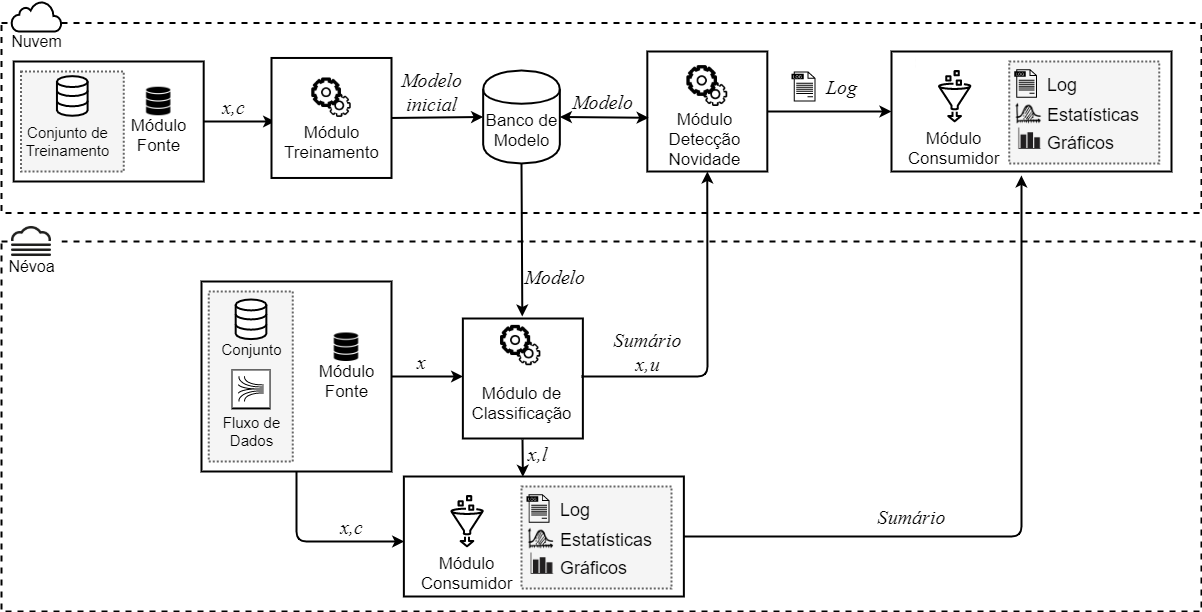
\includegraphics[width=1.1\textwidth]{../figuras/mfog-arch-v3_pt-br.png}
    \caption{Arquitetura e fluxos de dados do \mfog.}
    \label{fig:arch}
  \end{figure}
\end{frame}

\begin{frame}[fragile]{Método de Avaliação}
  \begin{alertblock}{Métricas e Ambientes}
    \begin{itemize}
      \item Métricas de qualidade de classificação:
      \begin{itemize}
        \item Avaliação do fluxo de saída do classificador;
        \item Uso de uma matriz de confusão ou erro;
        \item Taxa de desconhecidos;
        \item Macro F-score;
      \end{itemize}
    \end{itemize}
  \end{alertblock}

  \begin{columns}[T,onlytextwidth]
    \column{0.5\textwidth}
    \begin{equation*}
      \mathbf{E}_n = \begin{pmatrix}
        e_{1,1} & e_{1,2} & \cdots & e_{1,J} \\
        e_{2,1} & e_{2,2} & \cdots & e_{2,J} \\
        \vdots  & \vdots  & \ddots & \vdots  \\
        e_{M,1} & e_{M,2} & \cdots & e_{M,J} 
      \end{pmatrix}
    \end{equation*}

    % 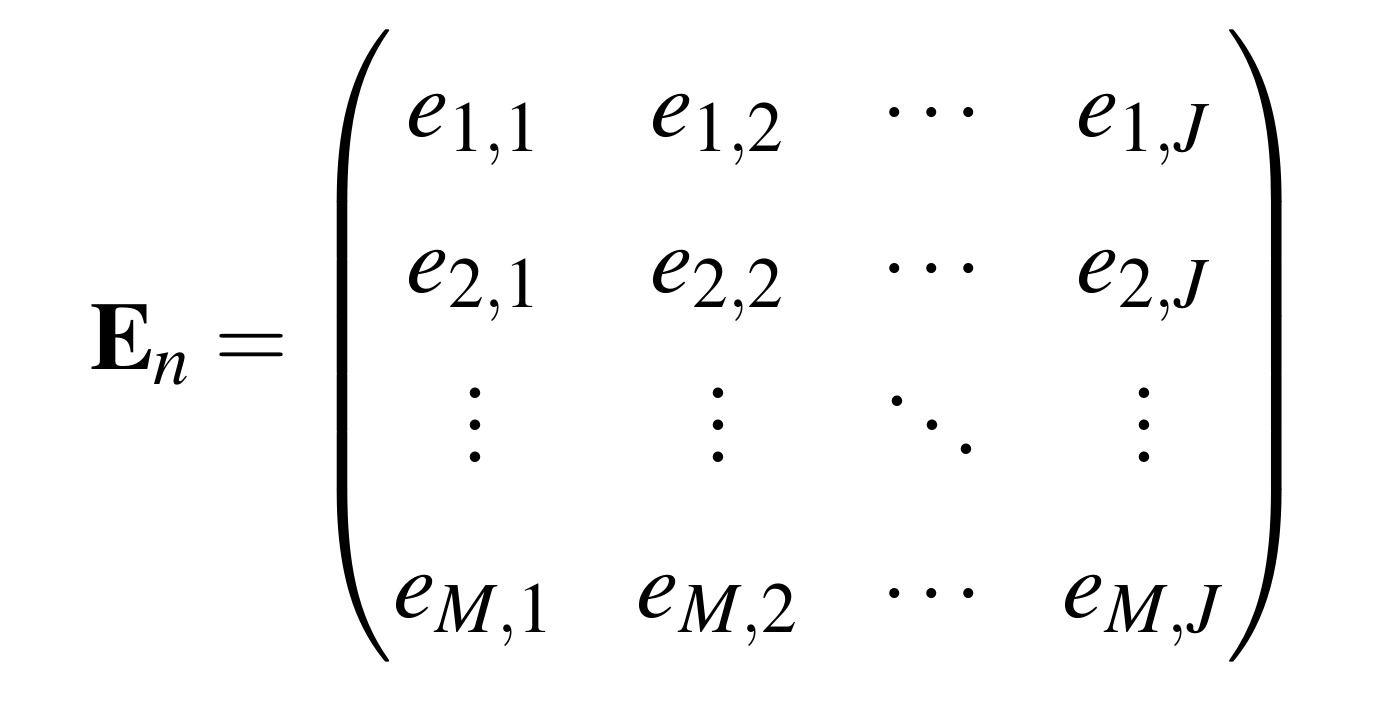
\includegraphics[width=0.9\textwidth]{figuras/eq-matrix.png}
    
    \column{0.5\textwidth}
    
    % 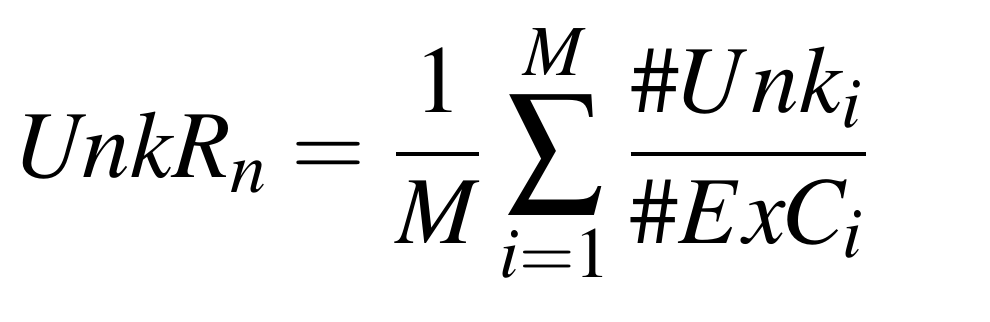
\includegraphics[width=0.9\textwidth]{figuras/eq-unk.png}
    % 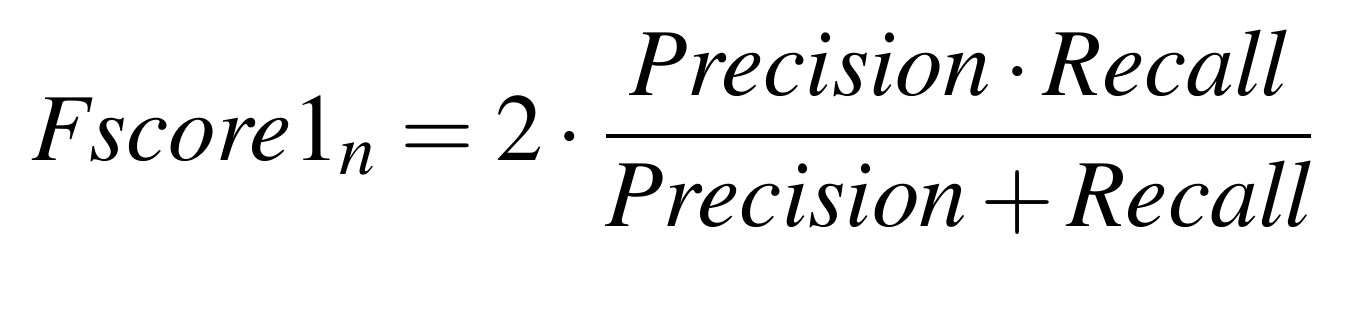
\includegraphics[width=0.9\textwidth]{figuras/eq-fscore1.png}
    
    \begin{equation*}
        \mathit{UnkR}_n      = \frac{1}{M} \sum_{i=1}^{M} \frac{\#Unk_i}{\#ExC_i} \\
        \mathit{Fscore}1_n   = 2 \cdot \frac{
          \mathit{Precision} \cdot \mathit{Recall}
          }{
            \mathit{Precision} +\mathit{Recall}
          }
    \end{equation*}
  \end{columns}
\end{frame}

\begin{frame}[fragile]{Método de Avaliação}

  Métricas de referência
  \vspace{0.5cm}
  
  \includegraphics[width=0.9\textwidth]{ref/Faria2015-CER-UnkR.png}
\end{frame}

\begin{frame}[fragile]{Método de Avaliação}
  \begin{alertblock}{Métricas e Ambientes}
    \begin{itemize}
      \item Métricas de escalabilidade:
      \begin{itemize}
        \item Número e tipo de processadores;
        \item Uso de memória;
        \item Tempo de processamento;
        \item Taxa de eventos;
        \item Latência entre a produção e classificação.
      \end{itemize}
      \item Ambientes de teste:
      \begin{itemize}
        \item Computador Pessoal (para desenvolvimento);
        \item Nuvem UFSCar;
        \item Nevoa composta de SBC (\emph{Sigle Board Computer}) ARM 4 núcleos;
      \end{itemize}
    \end{itemize}
  \end{alertblock}
\end{frame}


\section{Resultados Preliminares}
\begin{frame}[fragile]{Resultados Preliminares}

  \begin{alertblock}{Primeira Implementação com \emph{Python} e \emph{Apache Kafka}}
    \begin{itemize}%[<+- | alert@+>]
      \item \emph{Python} é acessível e fornece bibliotecas diversas;
      \item \emph{Apache Kafka} é um sistema de mensagens distribuído;
      \begin{itemize}
        \item Interface de programação com cliente produtor e consumidor;
        \item Mensagens organizadas em tópicos que são distribuídos em partições;
      \end{itemize}
      \item A hipótese de que a carga seria distribuída entre os consumidores,
      uma vez que o consumidor pode selecionar uma partição para leitura;
      \item Em experimento com um produtor, 8 partições e 8 consumidores,
      observou-se que um consumidor processava a maior parte das mensagens,
      poucos consumidores recebiam algumas mensagens e a maioria dos consumidores
      não recebia mensagem alguma.
    \end{itemize}
  \end{alertblock}
\end{frame}

\begin{frame}[fragile]{Resultados Preliminares}
  \begin{alertblock}{Segunda Implementação com \emph{Apache Flink}}
    \begin{itemize}%[<+- | alert@+>]
      \item Implementação escrita em Scala ou Java;
      \item Processamento de fluxos \emph{Stateful};
      \item Falta de bibliotecas que distribuam algoritmos base como \emph{K-means};
      \item Ambiente de execução (\emph{Flink Cluster}) consome mais memória do
      que disponível no \emph{hardware};
      \item Tempo de execução não foi melhor que a implementação original mesmo
      sem o trecho de detecção de novidades;
    \end{itemize}
  \end{alertblock}
\end{frame}

\begin{frame}[fragile]{Resultados Preliminares}
  \begin{alertblock}{Terceira Implementação com \emph{OpenMPI}}
    \begin{itemize}%[<+- | alert@+>]
      \item Implementação escrita em C;
      \item Versão serial e versão paralela e distribuída com \emph{MPI};
      \item Reimplementação de algoritmos base como \emph{K-means};
      \item Sistema \emph{M-FOG} em desenvolvimento, atualmente na fase de
      validação através das métricas de qualidade de classificação.
      \begin{itemize}
        \item Diferença entre os modelos iniciais gerados pelo algoritmo \emph{K-means};
        \item Diferença na matriz de confusão resultante da avaliação dos fluxos de saída;
      \end{itemize}
    \end{itemize}
  \end{alertblock}
\end{frame}

\begin{frame}[fragile]{Resultados Preliminares}
  \begin{alertblock}{Terceira Implementação com \emph{OpenMPI}}
    \includegraphics[width=1\textwidth]{ref/eval/speeup-chart.png}
  \end{alertblock}
\end{frame}

\begin{frame}[fragile]{Resultados Preliminares}
  \begin{alertblock}{Desafios Atuais}
    \begin{itemize}
      \item Diferença entre \texttt{double} e \texttt{float};
      \item Formato do fluxo de saída;
      \item Tratamento de exemplos com etiqueta \textit{desconhecido} utilizados
      para atualização do modelo;
      \item Diferença entre incluir ou não a borda do cluster;
      \item Definição de raio;
    \end{itemize}
  \end{alertblock}
\end{frame}

% ------------------------------------------------------------------------------

\section{Notas de Implementação}

\begin{frame}[fragile]{Algoritmo MINAS}
  \begin{alertblock}{Outras abordagens e implementações}
    \begin{itemize}%[<+- | alert@+>]
      \item FuzzyND por Da Silva 2018;
      \item Minas-LC e Minas-BR por Costa 2019;
      \item Implementação em Java por Douglas (douglas.m.cavalcanti@gmail.com) em Jul 2 09:37:42 2019
      \item Implementação em Python por Vitor Sexto Bernardes (vitorsb@gmail.com) em May 11 23:51:09 2020
    \end{itemize}
  \end{alertblock}
\end{frame}

\begin{frame}[fragile]{Algoritmo MINAS}
  \begin{alertblock}{Parâmetros}
    \includegraphics[width=1\textwidth]{ref/Faria2015-parameters.png}
  \end{alertblock}
\end{frame}

\begin{frame}[fragile]{Implementação referência}
  \begin{alertblock}{Parâmetros}
    % \includegraphics[width=1\textwidth]{ref/MINAS.java-params.png}
    \begin{Verbatim}[fontsize=\footnotesize]
class br.ufu.noveltydetection.minas.MinasOg with
	filenameOffline = datasets/training.csv
	filenameOnline = datasets/test.csv

	outputDirectory = out/minas-og//2020-07-20T12-18-21.758/
	algClusteringOff = kmeans
	algClusteringOnl = kmeans

	threshold = 2.0
	flagEvaluationType = 1
	thresholdForgettingPast = 10000
	numMicro = 100
	flagMicroClusters = true

	minExCluster = 20
	validationCriterion = dec

	skipNd = false
    \end{Verbatim}
  \end{alertblock}
\end{frame}
\begin{frame}[fragile]{Nova Implementação}
  \begin{alertblock}{Parâmetros}
    % \includegraphics[width=1\textwidth]{ref/MFOG-params.png}
    \begin{Verbatim}[fontsize=\small]
params->kParam = 100;
params->dimension = 22;
params->noveltyThreshold = 2;
params->minExCluster = 20;
params->maxUnkSize = params->kParam * params->minExCluster;
params->thresholdForgettingPast = 10000;
    \end{Verbatim}
  \end{alertblock}
\end{frame}

\begin{frame}[fragile]{Algoritmo MINAS}
  \begin{alertblock}{Fase offline}
    \includegraphics[width=1.1\textwidth]{ref/Faria2015-Alg1-Off.png}
  \end{alertblock}
\end{frame}

\begin{frame}[fragile]{Algoritmo MINAS}
  \begin{alertblock}{Final da fase offline, inicio da fase online}
    \begin{quotation}
    
      [\dots] N number of examples, LS linear sum of the examples, SS squared sum of the
      elements and T timestamp of the arrival of the last example classified in
      this micro-cluster.

      [\dots]
      After the execution of the clustering algorithm, each micro-cluster is
      represented by \alert{four components (N, LS, SS and T)}.
      
      [\dots]
      MINAS uses these measures to classify new examples. For such, it computes
      the distance between a new example and the closest centroid. If this
      distance is less than the micro-cluster radius, the example is classified
      
      [\dots]
      MINAS calculates the \alert{radius of a micro-cluster as the standard
      deviation} of the distance between the examples and the centroid, multiplied
      by a \alert{factor f}.
    
    \end{quotation}
  \end{alertblock}
\end{frame}

\begin{frame}[fragile]{Implementação referência}
  \begin{alertblock}{Fase Offline, definição de raio}
    \includegraphics[width=1\textwidth]{ref/MINAS.java-createKMeans.png}
    
    Detalhe:
    \includegraphics[width=1\textwidth]{ref/MINAS.java-createKMeans-detail.png}
  \end{alertblock}
\end{frame}
\begin{frame}[fragile]{Implementação referência}
  \begin{alertblock}{Fase Offline, definição de raio}
    \includegraphics[width=1\textwidth]{ref/MINAS.java-Kmeans.png}
  \end{alertblock}
\end{frame}
\begin{frame}[fragile]{Implementação referência}
  \includegraphics[width=1\textwidth]{ref/MINAS.java-Kmeans-radius2.png}
\end{frame}


\begin{frame}[fragile]{Algoritmo MINAS}
  \begin{alertblock}{Fase online}
    \includegraphics[width=1\textwidth]{ref/Faria2015-Alg2-On.png}
  \end{alertblock}
\end{frame}

\begin{frame}[fragile]{Implementação referência}
  \begin{alertblock}{Fase online}
    \includegraphics[width=1\textwidth]{ref/MINAS.java-identify.png}
  \end{alertblock}
\end{frame}

\begin{frame}[fragile]{Nova Implementação}
  \begin{alertblock}{Fase online}
    \includegraphics[width=1\textwidth]{ref/MFOG-identify.png}
  \end{alertblock}
\end{frame}

\begin{frame}[fragile]{Algoritmo MINAS}
  \begin{alertblock}{Fase online, Detecção de novidades}
    \includegraphics[width=1\textwidth]{ref/Faria2015-Alg3-ND.png}
  \end{alertblock}
\end{frame}

\begin{frame}[fragile]{Implementação referência}
  \begin{alertblock}{Output Stream}
    \includegraphics[width=1\textwidth]{ref/MINAS.java-outstream.png}
  \end{alertblock}
\end{frame}

\begin{frame}[fragile]{Nova Implementação}
  \begin{alertblock}{Output Stream}
    \includegraphics[width=1\textwidth]{ref/MFOG-outstream.png}
  \end{alertblock}
\end{frame}

\begin{frame}[fragile]{Implementação referência}
  \begin{alertblock}{Output Stream, Evaluation}
    \includegraphics[width=1\textwidth]{ref/MINAS.java-graph.png}
  \end{alertblock}
\end{frame}
\begin{frame}[fragile]{Implementação referência}
  \begin{alertblock}{Output Stream, Evaluation}
    \includegraphics[width=1\textwidth]{ref/MINAS.java-outstream-plot.png}
  \end{alertblock}
\end{frame}

\begin{frame}[fragile]{Nova Implementação}
  \begin{alertblock}{Output Stream, Evaluation}
    \includegraphics[width=1\textwidth]{ref/MFOG-outstream-plot.png}
  \end{alertblock}
\end{frame}

\begin{frame}[fragile]{Implementação referência}
  \begin{alertblock}{Matrix de confusão e avaliação}
    \includegraphics[width=1\textwidth]{ref/eval/MINAS.java-conf_mat.png}
  \end{alertblock}
\end{frame}
% Confusion Matrix
% Classes (act)       A       N assigned    hits  misses
% Labels (pred)                                         
% -                3774    8206        -       0       0
% 1                 123       0        A     123     123
% 10               3520    5130        N    5130    5130
% 11                 71     289        N     289     289
% 12                 26       0        A      26      26
% 2                 152      82        A     152     152
% 3                 368      44        A     368     368
% 4                   8       0        A       8       8
% 5                  82       1        A      82      82
% 6                 165       0        A     165     165
% 7                   8     396        N     396     396
% 8                1054     183        A    1054    1054
% 9                 161     154        A     161     161
% N              441395  199715        N  199715  199715
% Classes           ['A' 'N']
% Initial labels    ['-', 'N']
% Labels            ['-', '1', '10', '11', '12', '2', '3', '4', '5', '6', '7', '8', '9', 'N'] 14
% Total examples    (653457, 25)
% Total matches     (665107, 9)
% Hits               207669 ( 31.223397%)
% Misses             445458 ( 66.975389%)
% Unknowns            11980 (  1.801214%)
% Unk. reprocessed    11650 ( 97.245409%)
% Total              665107 (100.000000%)

\begin{frame}[fragile]{Nova Implementação}
  \begin{alertblock}{Matrix de confusão e avaliação}
    \includegraphics[width=1\textwidth]{ref/eval/MFOG-conf_mat.png}
  \end{alertblock}
\end{frame}
% \begin{frame}[fragile]{Nova Implementação}
%   \begin{alertblock}{Matrix de confusão e avaliação}
%     \begin{Verbatim}[fontsize=\tiny]
% Classes (act)       A       N assigned    hits  misses
% Labels (pred)                                         
% -                8306     355        -       0       0
% N              435763  205887        N  205887  205887
% a                 236       0        A     236     236
% b                 756      81        A     756     756
% c                 574       0        A     574     574
% d                 214       0        A     214     214
% e                 243       0        A     243     243
% f                 499       0        A     499     499
% g                 431       0        A     431     431
% h                 495       0        A     495     495
% i                 237       0        A     237     237
% j                 640       0        A     640     640
% k                  57       0        A      57      57
% l                 539       0        A     539     539
% m                  55       0        A      55      55
% n                  91       0        A      91      91
% o                  69       0        A      69      69
% p                3464       0        A    3464    3464
% q                 169       0        A     169     169
% r                 269       0        A     269     269
% Classes           ['A' 'N']
% Initial labels    ['-', 'N']
% Labels            ['-', 'N', 'a', 'b', 'c', 'd', 'e', 'f', 'g', 'h', 'i', 'j', 'k', 'l', 'm', 'n', 'o', 'p', 'q', 'r'] 20
% Total examples    (653457, 25)
% Total matches     (659430, 9)
% Hits               214925 ( 32.592542%)
% Misses             435844 ( 66.094051%)
% Unknowns             8661 (  1.313407%)
% Unk. reprocessed     5973 ( 68.964323%)
% Total              659430 (100.000000%)
%     \end{Verbatim}
%   \end{alertblock}
% \end{frame}

\begin{frame}[fragile]{Notas de Implementação}
  \begin{alertblock}{Algoritmo MINAS vs Implementação referência}
    \begin{itemize}%[<+- | alert@+>]
      \item Definição de raio: desvio padrão das distâncias versus distancia máxima;
      \item Atualização do micro-cluster limita-se à atualização do atributo \texttt{T};
      \item Remoção de exemplos na implementação de referência é feita somente para o algoritmo \textit{CluStream};
      \item Inclusão de borda: algoritmo inclui ($<=$), referência não inclui ($<$);
    \end{itemize}
  \end{alertblock}
\end{frame}
\begin{frame}[fragile]{Notas de Implementação}
  \begin{alertblock}{Algoritmo MINAS vs Nova Implementação}
    \begin{itemize}
      \item Seguiu-se as mesmas divergências anteriores para comparação dos resultados com a implementação referência;
      \item Inclusão da borda;
      \item Comportamento do mecânismo de \textit{sleep-model} não está definido, portanto não está ativo;
      \item Processo de clusterização é limitado ao algoritmo \textit{K-Means}. Algoritmo \textit{CluStream} não está implementado;
    \end{itemize}
  \end{alertblock}
\end{frame}



% \begin{frame}[fragile]{Algoritmo MINAS}
%   % MINAS \cite{Faria2016minas,Cassales2019a}
%   \begin{algorithm}[H]
%     \caption{MINAS, trecho de classificação}
%     \label{alg:MINAS}
%     \renewcommand{\algorithmicrequire}{\textbf{Entrada:}}
%     \begin{algorithmic}[1]
%       %T = limiar de distância para pertencer ao grupo
%       %P = tempo de "inatividade" para passar para memória sleep
%       %ts = limiar para remoção de exemplos da memória temporária
%       \REQUIRE $Modelo,FCD,params,MemTmp,MemSleep$
%       % \STATE $MemTmp \leftarrow \emptyset$ ; $MemSleep \leftarrow \emptyset$
%       \FORALL{$exemplo \in FCD$}
%       \STATE $(Dist,micro) \leftarrow$ micro-mais-proximo($exemplo,Modelo$)
%       \IF{$Dist < $ raio($micro$)}
%       \STATE $exemplo.classe \leftarrow micro.rotulo$
%       \STATE atualizar-micro($micro,exemplo$)
%       \ELSE
%       \STATE $exemplo.classe \leftarrow desconhecido$
%       \STATE $MemTmp \leftarrow MemTmp \cup exemplo$
%       \IF{$|MemTmp| \geq params.NumMinExemplos$}
%       \STATE $Modelo \leftarrow $ deteccao-novidade($Modelo,MemTmp,params$)
%       \ENDIF
%       \ENDIF
%       \STATE gerenciamento-memoria(\dots)
%       % \STATE $TempoAtual \leftarrow exemplo.T$
%       % \IF{$TempoAtual$ mod $TamJanela == 0$}
%       % \STATE $Modelo \leftarrow$ mover-micro-grupos-mem-sleep($Modelo,MemSleep,params$)
%       % \STATE $MemTmp \leftarrow$ remover-exemplos-antigos($MemTmp,params$)
%       % \ENDIF
%       \ENDFOR
%     \end{algorithmic}
%   \end{algorithm}
% \end{frame}

\end{document}
